\documentclass{article}
\usepackage[utf8]{inputenc}
\usepackage{amstext}
\usepackage{amsmath}
\usepackage{amsfonts}
\usepackage{graphicx}
\usepackage[margin=1in, paperwidth=8.5in, paperheight=11in]{geometry}
\usepackage{gensymb}
\usepackage{indentfirst}
\usepackage{textcomp}
\usepackage{upgreek }
\usepackage{siunitx}
\usepackage{enumitem}
\usepackage{epstopdf}
\usepackage{float}
\epstopdfsetup{update} % only regenerate pdf files when eps file is newer

\usepackage[american]{circuitikz}

\title{Adaptive-Biasing Differential Amplifier}
\author{Byron Wasti}
\date{May 2017}

\begin{document}
\maketitle

\section{Background}

    The differential amplifiers we have been studying in Circuits have a number of properties that we have been steadily improving. For instance, rail-to-rail common-mode input and rail-to-rail output were two additions to the basic differential amplifier we started with. This project looks to improve the slew-rate of differential amplifier from Postlab 9.

    There are a number of strategies for improving the slew-rate, but I decided to look at using an adaptive-biasing approach with subtractor sub-circuits. This idea came from the suggested reading, M.  G.  Degrauwe,  J.  Rijmenants, E. A. Vittoz, and H. J. de Man, “Adaptive Biasing CMOS Amplifiers,” \textit{IEEE Journal of Solid-State Circuits}, vol. SC-17, no. 3, pp. 522–528, 1982.

    The general idea is to modify the input stage of the differential amplifier to adaptively change the current drawn by the bias transistor based on the difference between the input voltages. Due to KCL, $I_b = I_1 + I_2$. From our analysis in class, the output voltage of the differential amplifier occurs when $I_1 = I_2$, which during a large-step input happens when either the $p$MOS or the $n$MOS in the output stage goes into the ohmic region. Thus, by increasing $I_1$ or $I_2$ we can increase the rate at which the parasitic capacitance charges or discharges (and thus brings up the voltage or lowers it). Due to the direct relationship between $I_1$, $I_2$ and $I_b$, by increasing $I_b$, or the virtual $I_b$, when $I_1$ and $I_2$ are very different, we can increase the rate at which the differential amplifier reaches either rail (ie. The slew rate).

    To calculate this difference, we will use a subtractor circuit. In order to increase $I_b$, we will add transistors in parallel which will sink additional current when $I_1$ and $I_2$ differ by a significant amount.
    
\section{Subtraction Sub-Circuit}

    To begin the analysis of the adaptive-biasing differential amplifier, we first have to understand the operating regions of the subtractor circuit. A schematic for the subtractor circuit can be found in Figure \ref{fig:subtractor_schem}. This circuit is rather easy to analyze, as $I_1$ is mirrored such that the mirroring transistor sinks $I_2$. Any current not sunk by the mirrored-$I_1$ transistor then goes through another current mirror, which is the output current. Thus, the output current is a scaled $I_2 - I_1$ (it is scaled due to the Early effect, but this is not very important) except it is limited because it cannot go below $0$A. This is because if $I_1 \ge I_2$, then all of the current for $I_2$ will go through the transistor mirroring $I_1$'s current due to KCL.

    The current transfer characteristic for the subtractor circuit can be seen in Figure \ref{fig:subtractor_input}, where it can be seen that if $I_1 \ge I_2$ the output current goes to $0$A.

    Due to the limitation of the subtraction circuit not going below $0$A, we will need at least two in our final adaptive-biasing differential amplifier. One to calculate $I_2 - I_1$, and another to calculate $I_1 - I_2$. 

    \begin{figure}[htp]
        \centering
        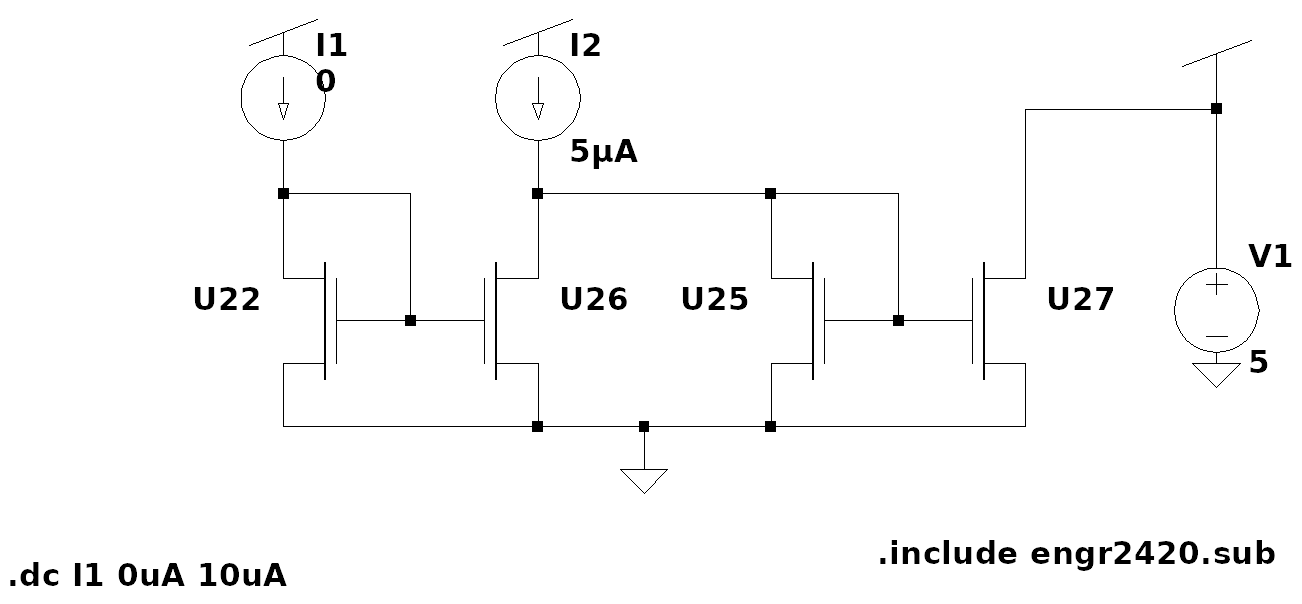
\includegraphics[width=\textwidth]{../Plots/subtractor_schem.png}
        \caption{Subtractor schematic to be used in the adaptive-biasing differential amplifier.}
        \label{fig:subtractor_schem}
    \end{figure}

    \begin{figure}[htp]
        \centering
        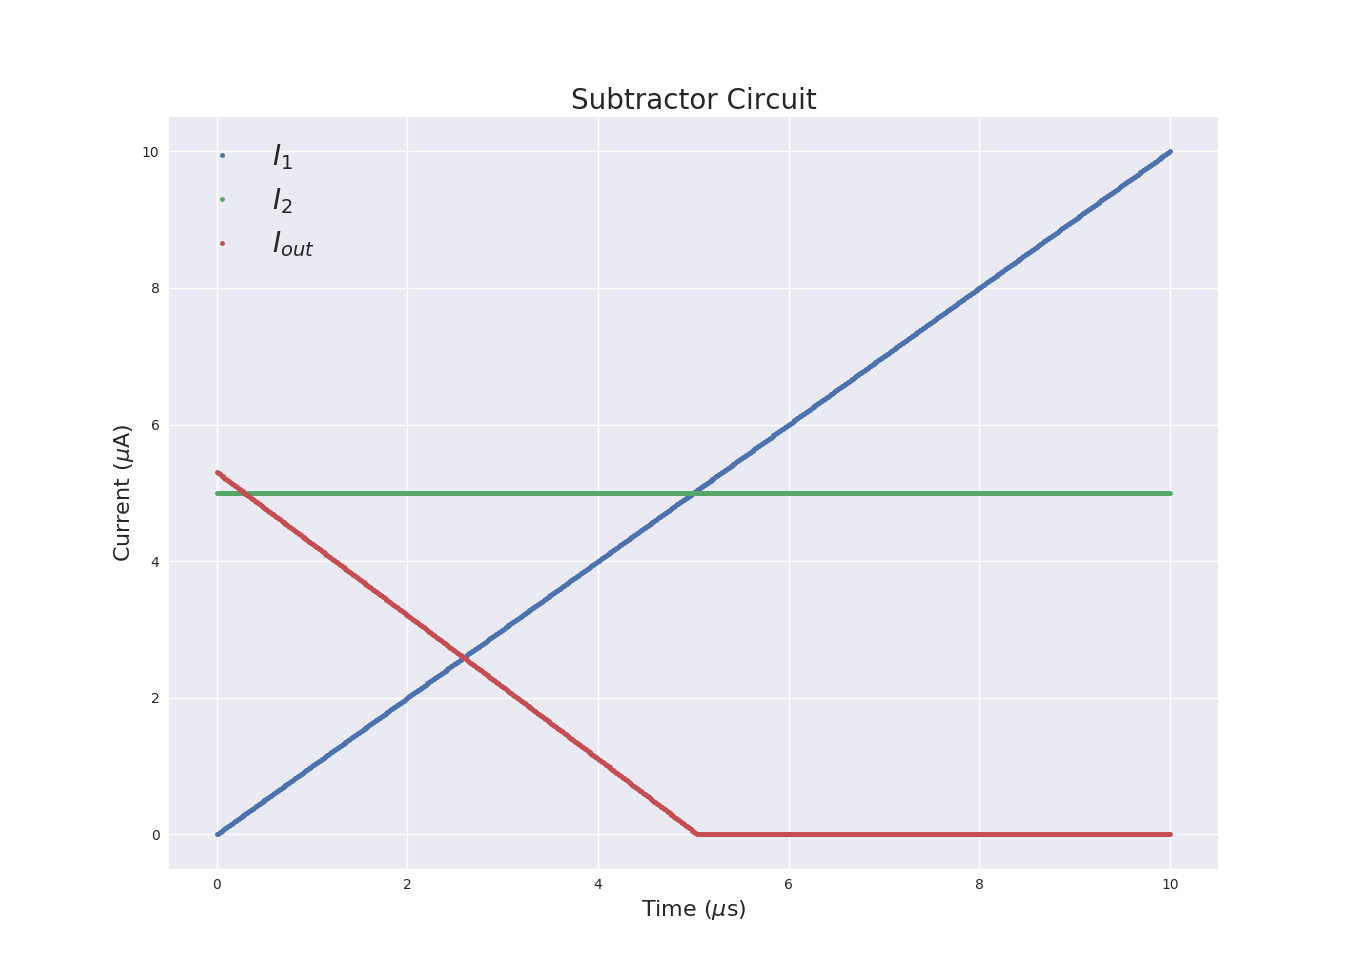
\includegraphics[width=\textwidth]{../Plots/subtractor.png}
        \caption{Subtractor circuit input response.  Note that the output is a slightly scaled $I_2 - I_1$, but cannot go below $0$A.}
        \label{fig:subtractor_input}
    \end{figure}


\newpage
\section{Adaptive-Biasing Differential Amplifier}

    The next step is to modify our differential amplifier from Postlab 9 with the subtractor circuit mentioned above in order to make the adaptive-biasing differential amplifier. The adaptive-biasing differential amplifier schematic can be seen in Figure \ref{fig:schematic-adaptive}.

    Due to the way the differential amplifier was constructed in Postlab 9, there were a few additional stages that were required to be added in order to mirror the input currents for the subtractor circuits.The output current of the subtractor circuits is also mirrored with a $p$MOS mirror so that the $p$MOS differential input stage can adaptively bias as well.

    \begin{figure}[h]
        \centering
        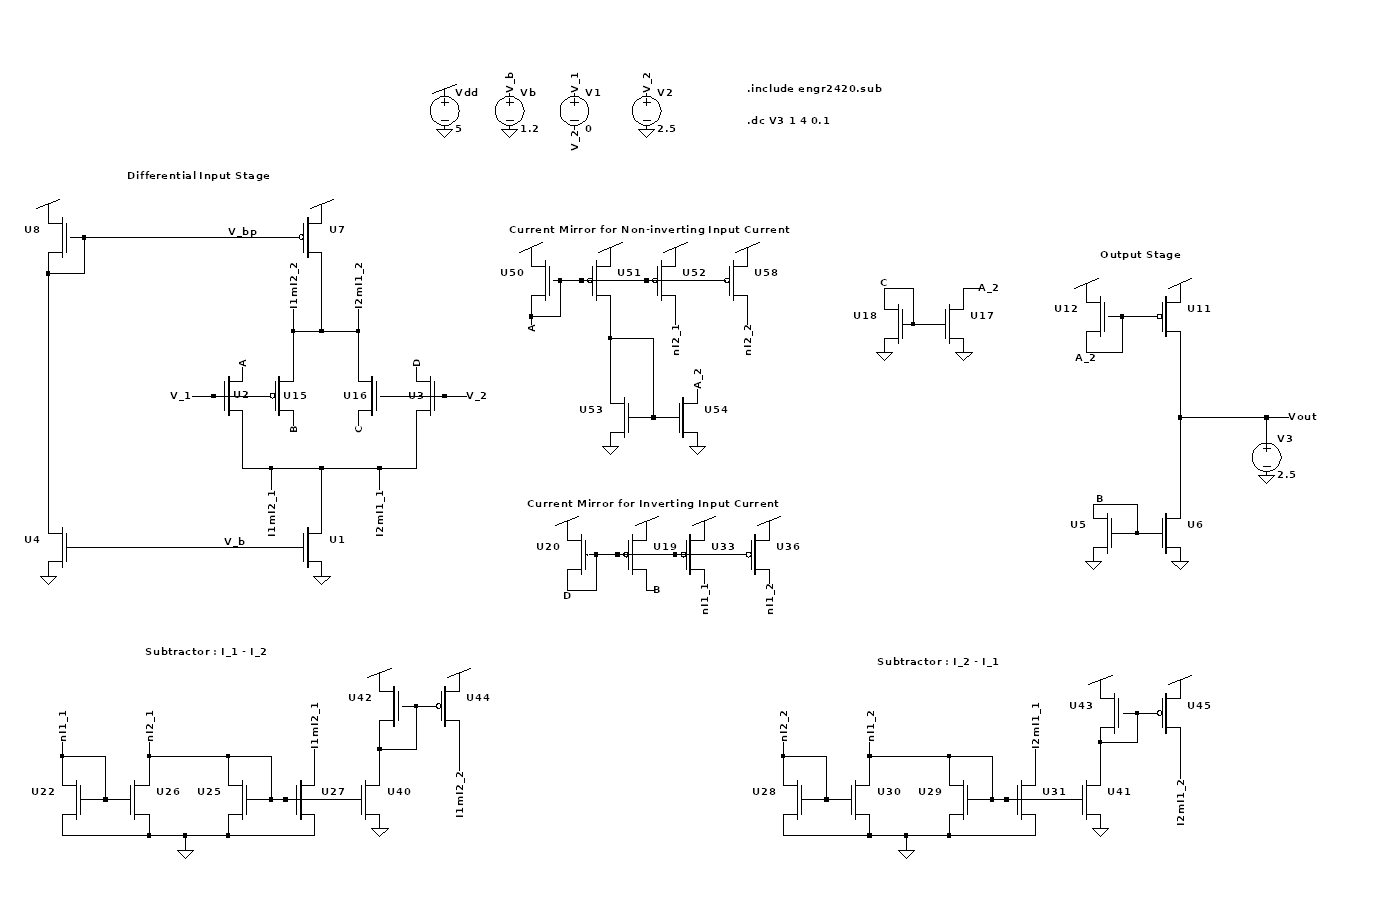
\includegraphics[width=\textwidth]{../Plots/adaptive-biasing-schematic.png}
        \caption{Adaptive-biasing Differential Amplifier. There are two subtractor circuits used which adaptively bias the differential input stage.}
        \label{fig:schematic-adaptive}
    \end{figure}


\newpage
\section{Voltage Transfer Characteristic}

    The voltage transfer characteristic for the adaptive-biasing differential amplifier is shown in Figure \ref{fig:VTC}. The voltage transfer characteristic shows that the differential amplifier is still rail-to-rail common-mode input and rail-to-rail output swing. However, the differential amplifier is not perfect, and the rail-to-rail output swing does not reach either rail exactly. This is definitely a problem with the design as is, but for now we only care about the adaptive-biasing.

    \begin{figure}[h]
        \centering
        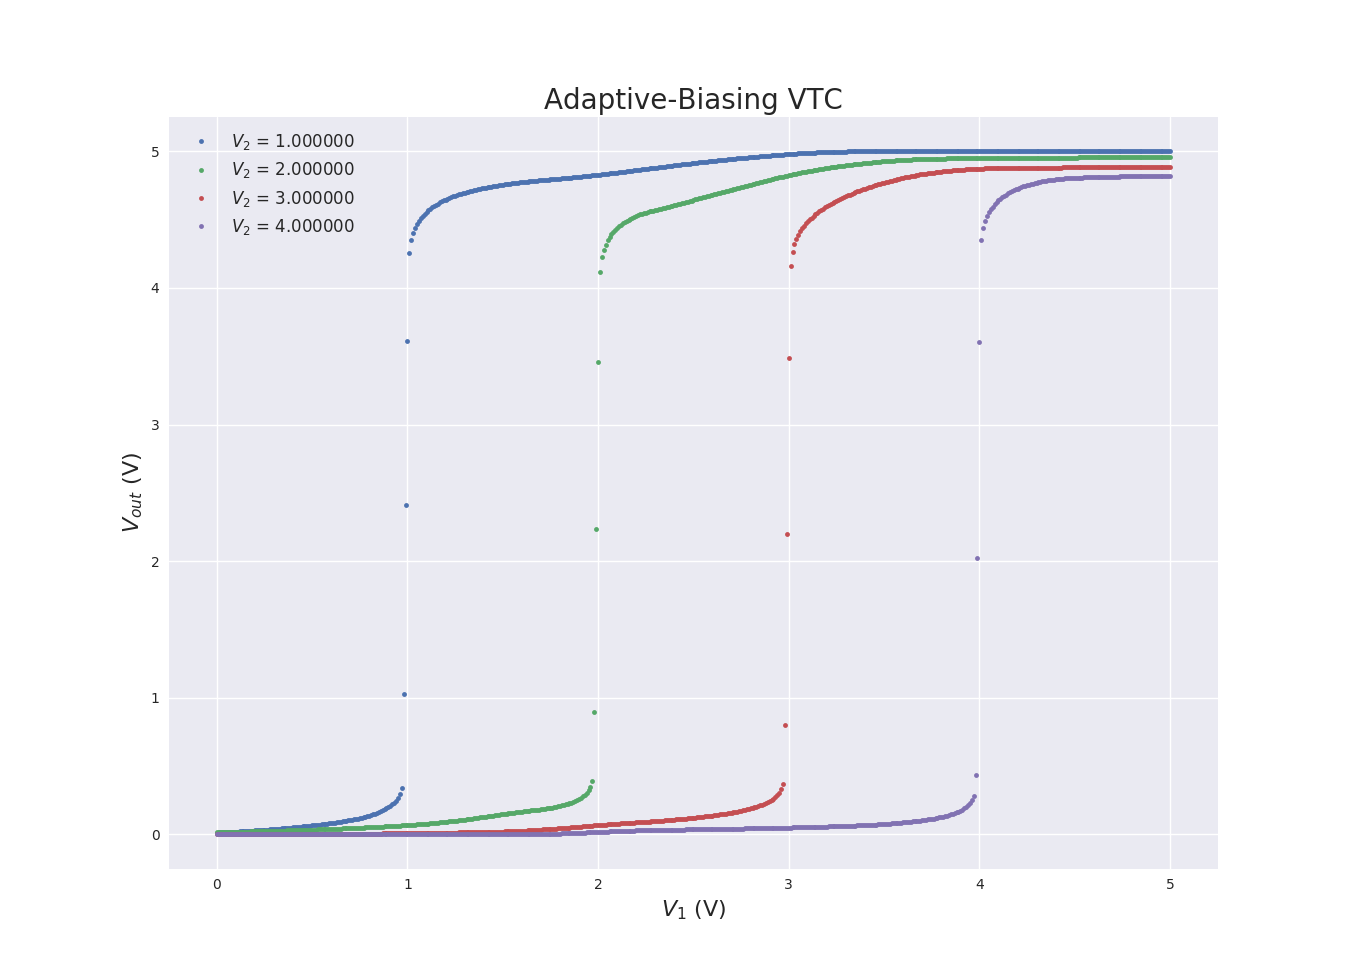
\includegraphics[width=\textwidth]{../Plots/VTC.png}
        \caption{Voltage transfer characteristic for the adaptive-biasing differential amplifier.}
        \label{fig:VTC}
    \end{figure}


\newpage
\section{Differential-Mode Gain}

    There are two methods to calculate the differential-mode gain of the differential amplifier. One is simply finding the slope of $V_{out}$ vs. $V_{dm}$. The other is finding the output resistance and the transconductance of the circuit, and knowing that $A_{dm} = G_{m}R_{out}$. 

    \subsection{$V_{out}$ vs. $V_{dm}$}

        The first method for calculating the differential-mode gain is to find the slope of $V_{out}$ vs. $V_{dm}$ where it is steepest. From Figure \ref{fig:diffModeGain}, one can see that the extracted slope is $118.396$. Thus, $A_{dm} \approx 118.396$.

        \begin{figure}[h]
            \centering
            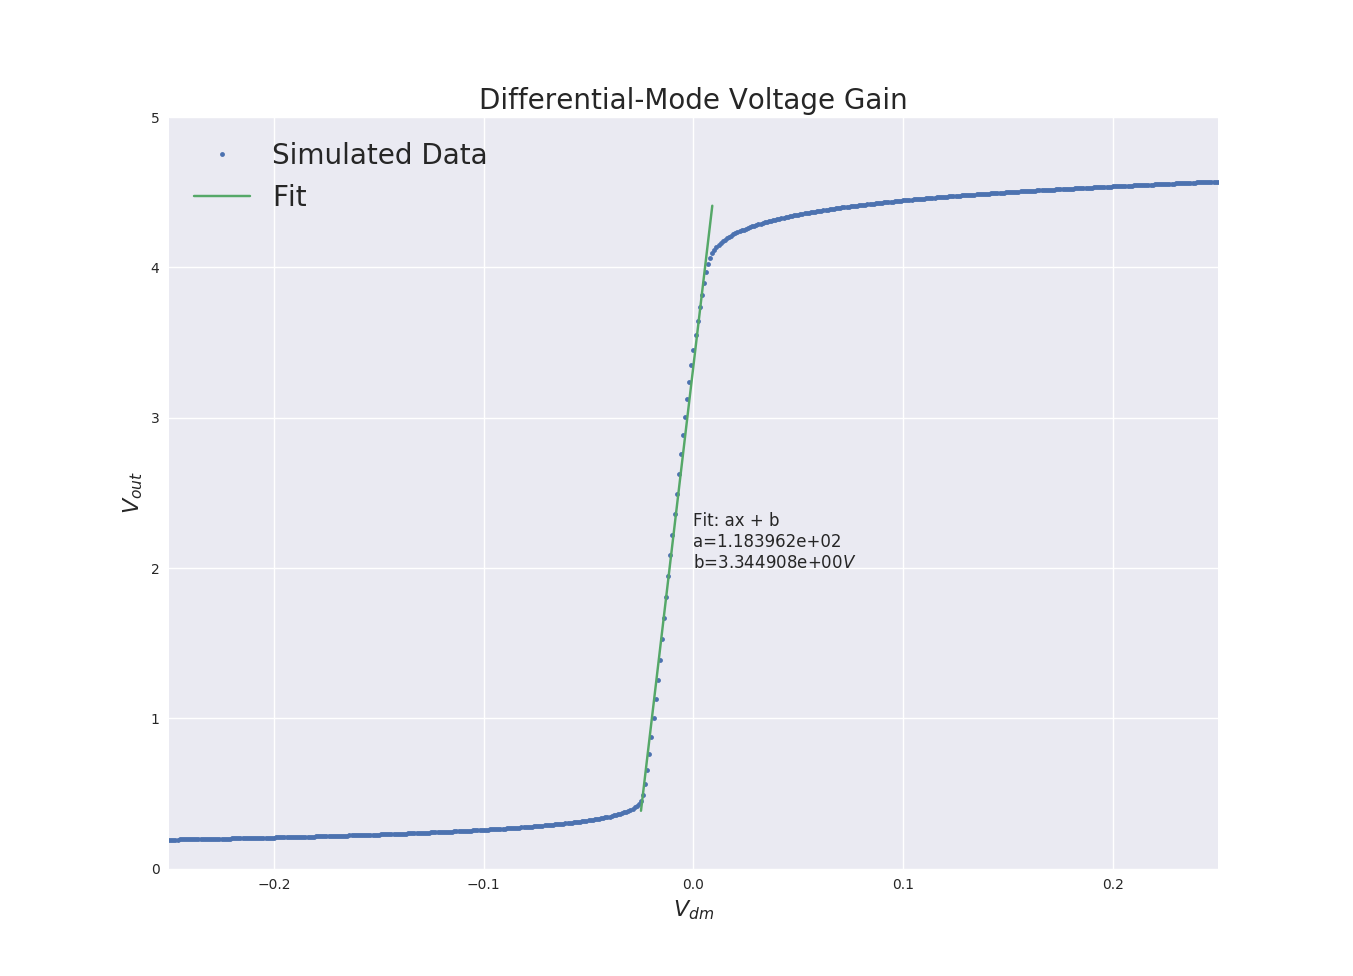
\includegraphics[width=\textwidth]{../Plots/diffModeGain.png}
            \caption{Differential-mode gain extracted from the slope of $V_{out}$ vs $V_{dm}$.}
            \label{fig:diffModeGain}
        \end{figure}


    \subsection{$A_{dm} = G_{m}R_{out}$}
        The second method for finding the differential-mode gain is to find the output resistance and the transconductance and taking their product, since $A_{dm} = R_{out}G_{m}$. To find the output resistance, we can look at one over the slope of $I_{out}$ vs. $V_{out}$, which can be seen in Figure \ref{fig:outputRes}. We get a value for $R_{out} = 2.641430e06$.

        To find the transconductance, we simply look at the slope for $I_{out}$ vs. $V_{dm}$, since $\delta I_{out} / \delta V_{dm} \approx G_{m}$. As shown in Figure \ref{fig:transconductance}, the line is not linear which means this approximation is not very accurate. The reason the line varies so much is due to the dual-input stage ($p$MOS and $n$MOS), where near the middle of the operation region of the differential-amplifier are both active. Thus, the $G_{m}$ is not close to constant throughout the operating regions of the differential amplifier. However, doing our best, we get a value for $G_{m} = 7.25e-05$. Note that even though the plot does not show a straight line, the general slope of the fit still gives a reasonable value.

        Thus, we find that $A_{dm} \approx 191.5$, which is almost double the value we found before. However, this error can probably be attributed to the transconductance approximation being rather sketchy.

        \begin{figure}[h!]
            \centering
            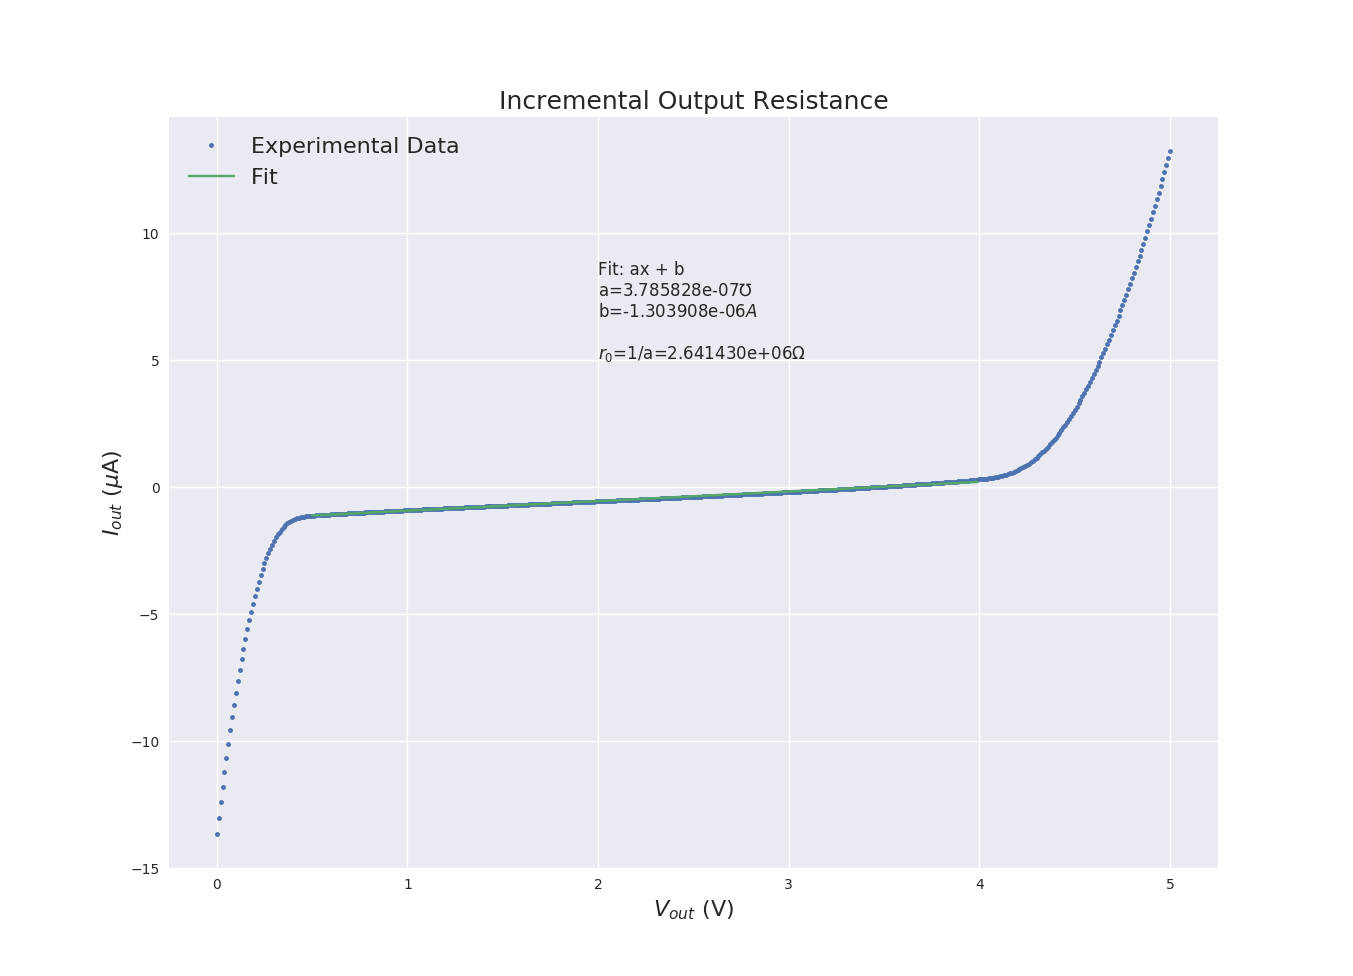
\includegraphics[width=0.8\textwidth]{../Plots/outputResistance.png}
            \caption{Output resistance for the adaptive-biasing circuit.}
            \label{fig:outputRes}
        \end{figure}

        \begin{figure}[h!]
            \centering
            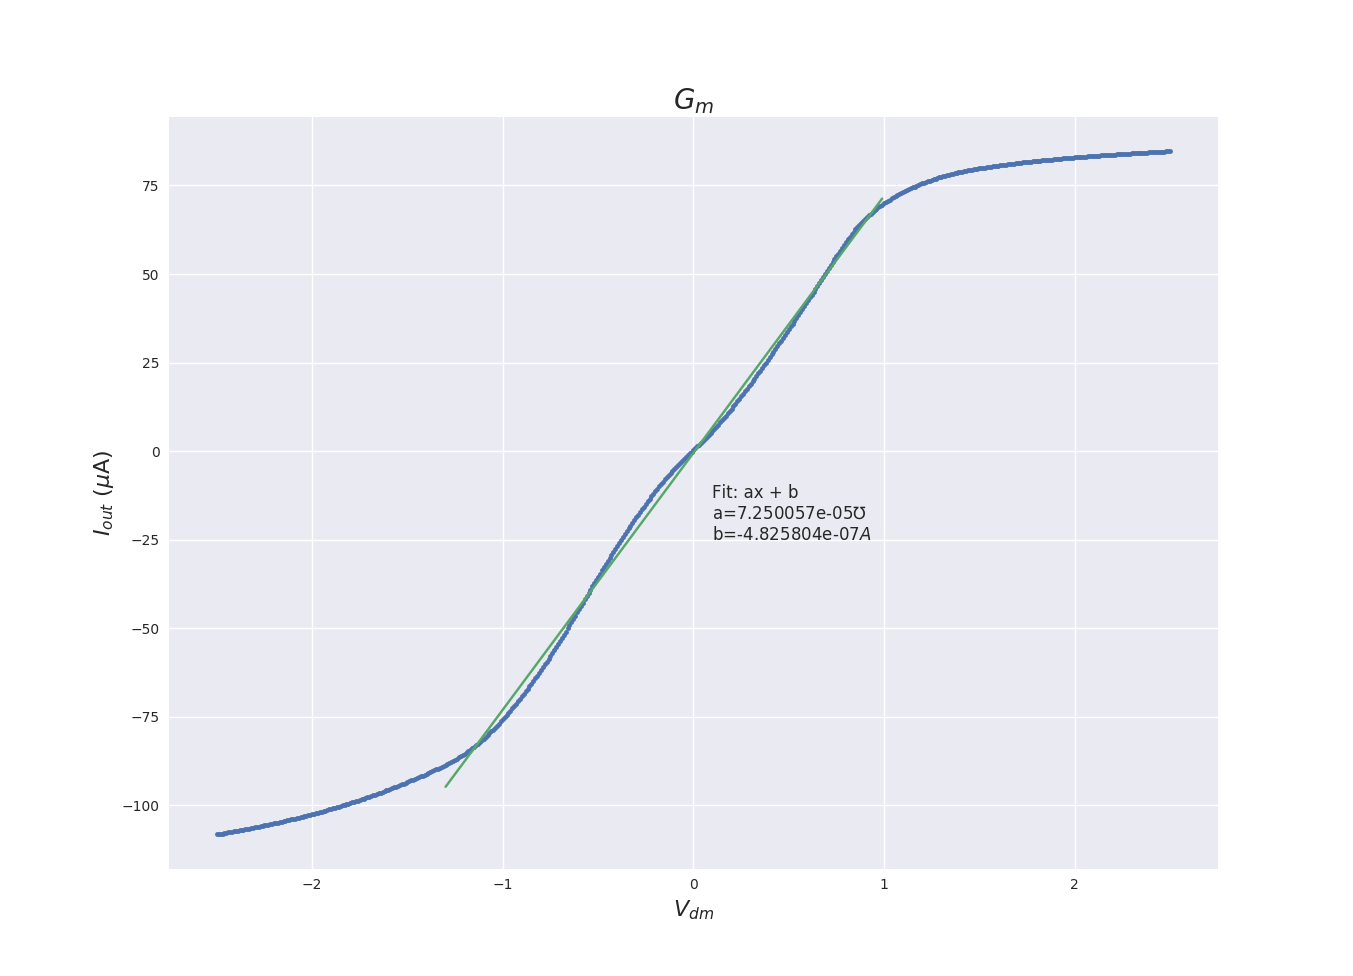
\includegraphics[width=0.8\textwidth]{../Plots/transconductanceGain.png}
            \caption{Transconductance extracted for the adaptive-biasing circuit}
            \label{fig:transconductance}
        \end{figure}

\section{Slew Rate Comparison}

    The goal of the adaptive-biasing circuit is to dramatically increase the slew-rate of the differential amplifier. Figure \ref{fig:slew_rate} shows the comparison between the Postlab 9 circuit and the adaptive-biasing circuit. As can be seen from the extracted slew-rates, the slew-rate of the adaptive-biasing differential amplifier has an increase of about an order of magnitude. This is good, and proves that our theory is valid.

    \begin{figure}[h]
        \centering
        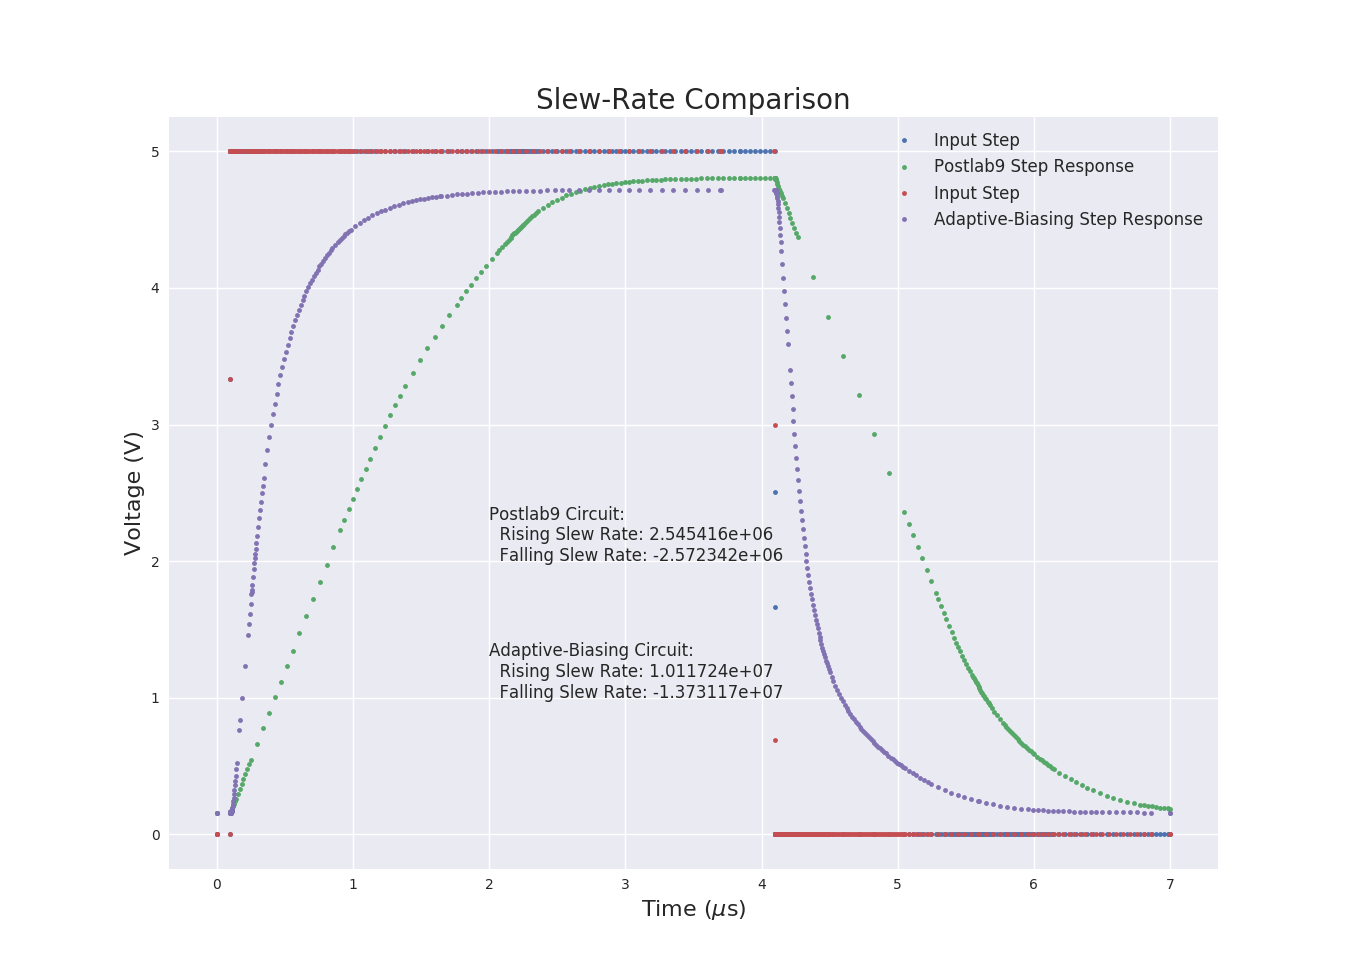
\includegraphics[width=\textwidth]{../Plots/slew_rate.png}
        \caption{Rising and Falling slew rate comparison for the adaptive-biasing circuit compared to the previous rail-to-rail common-mode differential amplifier from Postlab 9.}
        \label{fig:slew_rate}
    \end{figure}


\section{Conclusion and Further Research}

    The adaptive-biasing addition to the differential amplifier increases the slew rate by about an order of magnitude, which means it functions as expected. We could most likely increase the slew rate more by adjusting the power-ratios of the subtractor circuit's output stage to sink a higher proportion of current when $I_1$ and $I_2$ are significantly different from each other. However, the adaptive-biasing differential amplifier proves the concept of adaptive biasing.

    One of the largest downsides with the current design are the variable $G_{m}$ (and thus, $A_{dm}$) as well as the non-perfect rail-to-rail operation. Further refinements of the design would help fix these problems, such as modifying the power-ratios of the transistors in the differential amplifier.


\end{document}
